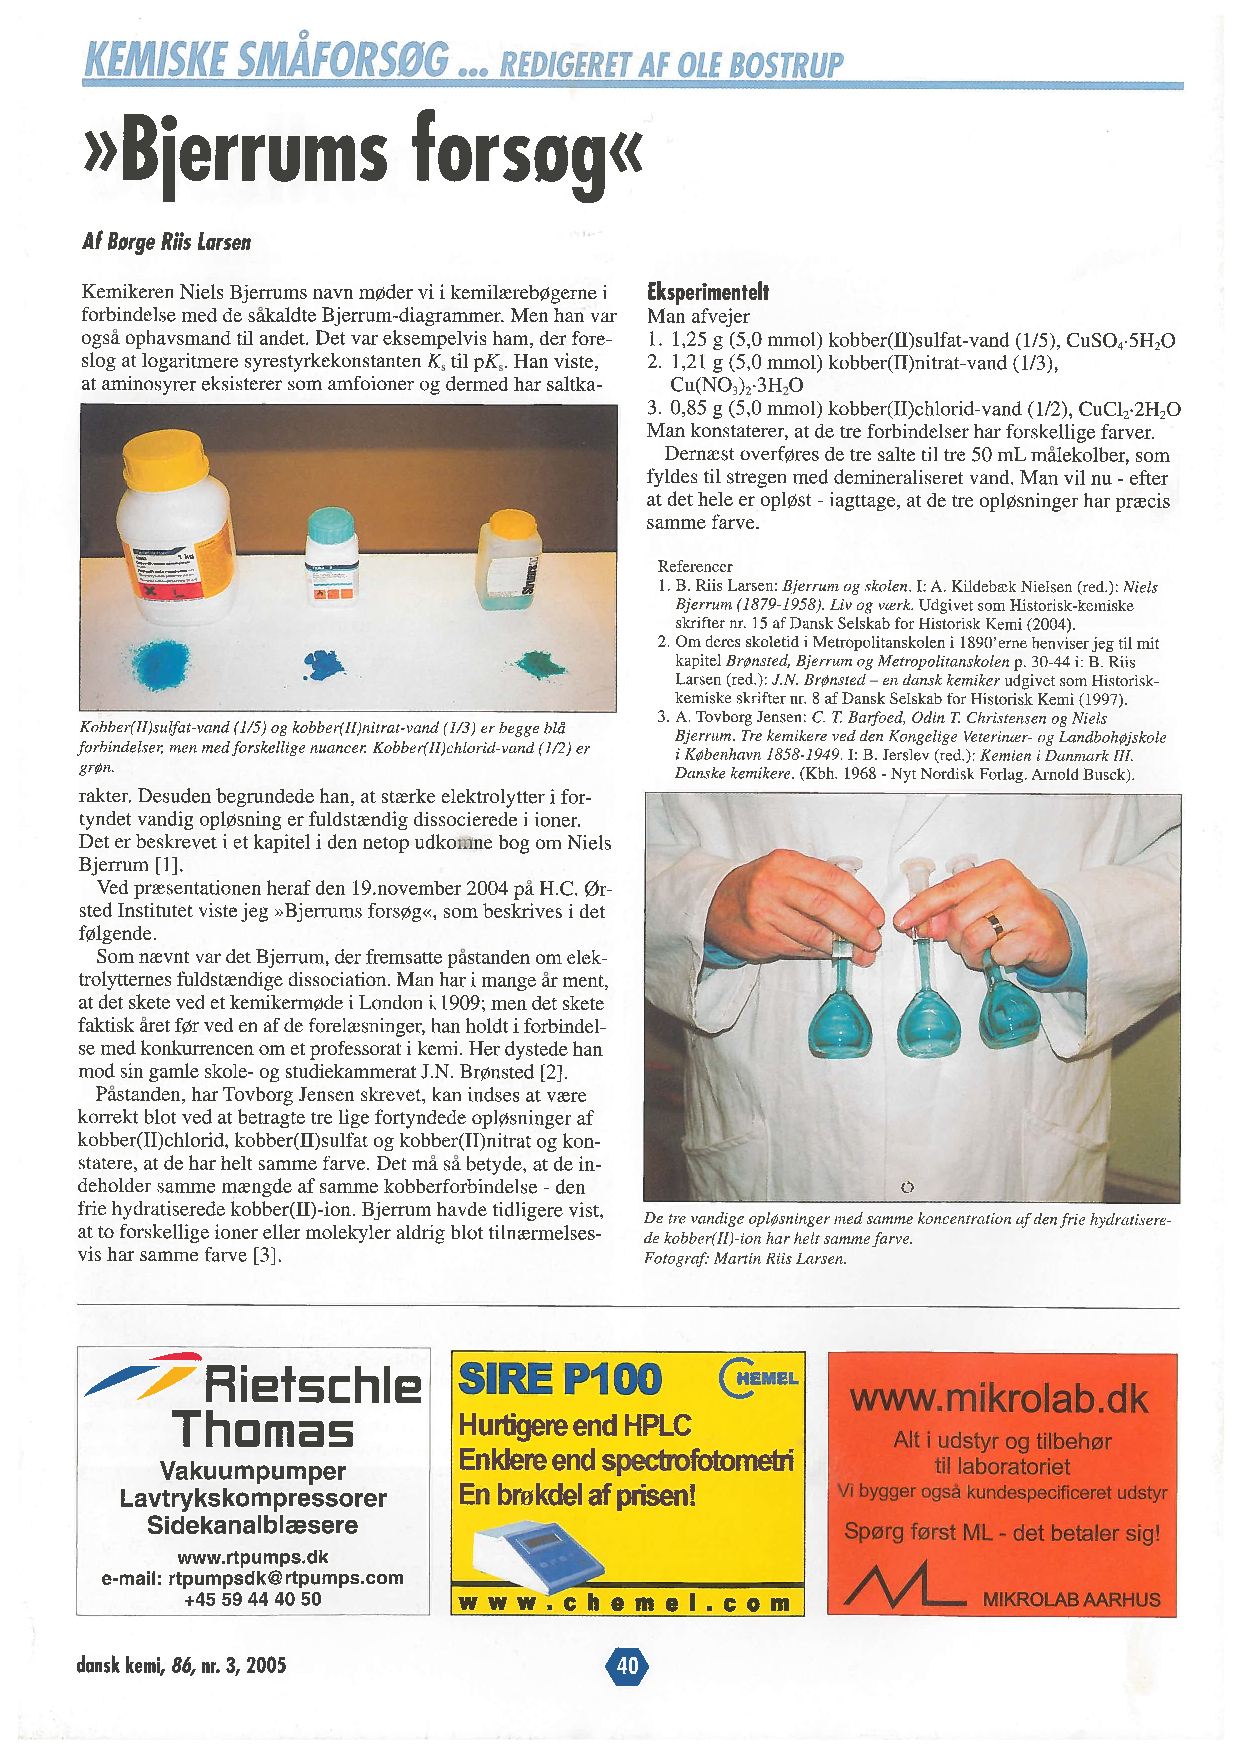
\includepdf[pages=-]{pdfs/2005-86-3-40.pdf}

\emne{"Bjerrums forsøg"}
\danskkemi{Dansk Kemi 86, 3, 2005, p. 40}

Af Børge Riis Larsen

Kemikeren Niels Bjerrums navn møder vi i kemilærebøgerne i forbindelse med de
såkaldte Bjerrum-diagrammer. Men han var også ophavsmand til andet. Det var
eksempelvis ham, der foreslog at logaritmere syrestyrkekonstanten $K_{s}$
til $pK_{s}$.
Han viste at aminosyrer eksisterer som amfoioner og dermed har saltkarakter.
Desuden begrundede han, at stærke elektrolytter i fortyndet vandig opløsning
er fuldstændig dissocierede i ioner. Det er beskrevet i et kapitel i den netop
udkomne bog om Niels Bjerrum [1].

Ved præsentationen heraf den 19. november 2004 på H.C. Ørsted Institutet viste
jeg "Bjerrums forsøg", som beskrives i det følgende.

Som nævnt var det Bjerrum, der fremsatte påstanden om elektrolytternes
fuldstændige dissociation. Man har i mange år ment, at det skete ved et
kemikermøde i London i 1909; men det skete faktisk året før ved en af de
forelæsninger, han holdt i forbindelse med konkurrencen om et professorat i
kemi. Her dystede han mod sin gamle skole- og studiekammerat J.N. Brønsted [2].

Påstanden, har Tovborg Jensen skrevet, kan indses at være korrekt blot ved at
betragte tre lige fortyndede opløsninger af kobber(II)chlorid, kobber(II)sulfat
og kobber(II)nitrat og konstatere, at de har helt samme farve. Det må så betyde,
at de indeholder samme mængde af samme kobberforbindelse - den frie hydratiserede
kobber(II)-ion. Bjerrum havde tidligere vist, at to forskellige ioner eller
molekyler aldrig blot tilnærmelsesvis har samme farve [3].


\deloverskrift{Eksperimentelt}


Man afvejer

1. 1,25 g (5,0 mmol) kobber(II)sulfat-vand (1/5), \ch{CuSO4}$\cdotp$\ch{5 H2O}

2. 1,21 g (5,0 mmol) kobber(II)nitrat-vand (1/3), \ch{Cu(NO3)2}$\cdotp$\ch{3 H2O}

3. 0.85 g (5,0 mmol) kobber(II)chlorid-vand (1/2), \ch{CuCl2}$\cdotp$\ch{2 H2O}

Man konstaterer, at de tre forbindelser har forskellige farver.

Dernæst overføres de tre salte til tre 50 mL målekolber, som fyldes til stregen
med demineraliseret vand. Man vil nu - efter at det hele er opløst - iagttage,
at de tre opløsninger har præcis samme farve.

Referencer
1. B. Riis Larsen: Bjerrum og skolen. I A. Kildebæk Nielsen (red.): Niels Bjerrum
(1879-1958). Liv og værk. Udgivet som Historisk-kemiske skrifter nr. 15 af Dansk
Selskab for Historisk Kemi (2004).
2. Om deres skoletid i Metropolitanskolen i 1890'erne henviser jeg til mit
kapitel Brønsted, Bjerrum og Metropolitanskolen p. 30-40 i: B. Riis Larsen (red.):
J.N. Brønsted - en dansk kemiker udgivet som Historisk-kemiske skrifter nr. 8
af Dansk Selskab for Historisk Kemi (1997).
3. A. Tovborg Jensen: C.T. Barfoed, Odin T. Christensen og Niels Bjerrum. Tre
kemikere ved den Kongelige Veterinær- og Landbohøjskole i København 1858-1949. I:
B. Jerslev (red.): Kemien i Danmark III. Danske Kemikere. (Kbh. 1968 - Nyt Nordisk
Forlag. Arnold Busck).
